\documentclass[12pt,fleqn]{article}\usepackage{../../common}
\begin{document}
Paralel KMeans, Hadoop

K-Means algoritmasını nasıl paralel şekilde işletiriz? Özellikle Hadoop gibi bir
Eşle-İndirge (Map-Reduce) ortamını düşünelim. Veri çok büyük ölçekte olabilir ve
bu veriler birden fazla makinaya bölünecektir. Eşle-İndirge kavramında eşleme
safhasında "anahtar üretiriz", ve sonra indirgeme safhasında Hadoop sistemi öyle
kurmuştur ki aynı anahtarlarlar tek bir makinaya gönderilir, ve bu nihai aşamada
artık anahtar bazında indirgeme (özetleme) yapılır.

Paralel K-Means için anahtar nedir? Anahtar, mesela küme olabilir. Yani
küme 1, küme 2 gibi küme işaretleri / sayıları anahtar olarak
kullanılabilirler.

Peki anahtar ile eşlenecek "değer" nedir?

Öyle bir değer arıyoruz ki üst üste konulabilecek bir şey olmalı, Eİ sisteminin
kuvveti burada, anahtarlar farklı noktalarda üretilebiliyor, sonra tek noktada
üst üste konuyor, o zaman değerler öyle üretilmeli ki bu üst üste koyma,
özetleme işlemi yapılabilsin. Üst üste konabilecek şey, her veri noktası için, o
veri noktasının ait olduğu küme üzerinden toplama işlemidir. 10.20, 20.5 veri
noktasına bakıyorum, bu nokta o anda elde olan küme merkezlerinden 6'ya en
yakın, 10.20, 20.5 verisi ile bir 6 anahtarı yayınlarım.

Tabii burada tavuk/yumurta problemi var, küme merkezlerini arıyorum, ama
anahtar üretimi için küme merkezi lazım. Bu nasıl olacak?  O zaman (ilk
başta rasgele bile olsa) küme merkezlerinin bilgisi tüm makinaların
erişebileceği bir yerde olmalı. Biz bu veriyi \verb!centers.csv!  adlı bir
dosyaya koymaya karar verdik, bu dosya tek makina ortamında bilinen bir
dizinde (mesela /tmp), çok makinalı ortamda ise HDFS üzerinde herkesin
erişebileceği bir yerde olmalı.

Toplamaya gelelim: Normal K-Means'i hatırlarsak, her nokta için o noktaya
en yakın kümeyi buluyordu ve sonra, atama işlemi bitince, her kümenin
altındaki noktaları toparlayıp onların ortalamasını alarak yeni küme
merkezini hesaplıyordu. Paralel ortamda ortalama işlemi üst üste
konabilecek bir şey, çünkü toplama üst üste konabilecek bir işlem, ve /
yani farklı makinalarda küme-nokta, eşlemelerini üretirsek, indirgeme
aşamasında o anahtar için tüm değerleri toplayıp nokta sayısına böleriz ve
yeni küme merkezini elde ederiz.

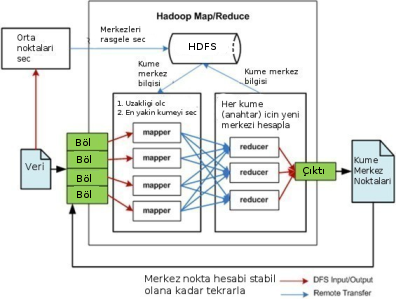
\includegraphics[height=8cm]{kmeans-diag.png}

Şimdi Hadoop ile ilgili bazı lojistik konulara gelelim:

Paralel K-Means için tek bir eşle-indirge işletimi yeterli değil, bu algoritma
döngülü / özyineli (iterative) bir algoritma, 5,10,20 kez işlemesi gerekebilir.
Her döngü (indirgeme) sonunda yeni küme merkezleri hesaplanacak, bu merkezler
eski \verb!centers.csv!  yerini alacak ve işlem tekrar başlayacak.

Şimdi ham veriyi gösterelim,

\begin{minted}[fontsize=\footnotesize]{python}
from pandas import *
df1 = read_csv("../kmeans/synthetic.txt",comment='#',,sep="   ")
plt.scatter(df1.ix[:,0],df1.ix[:,1])
plt.savefig('kmeans_1.png')
\end{minted}

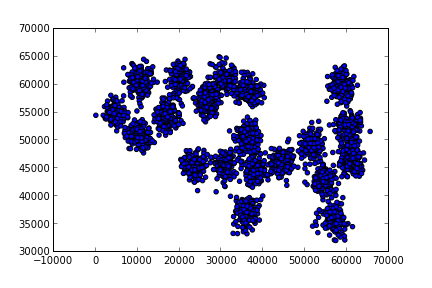
\includegraphics[height=4cm]{kmeans_1.png}

\inputminted[fontsize=\footnotesize]{python}{kmeans.py}

\verb!reduce_all_centers! çağrısı tüm indirgeyiciler her küme için yeni
orta noktayı hesaplayıp onu yayınladıktan (emit) sonra, tüm yeni
merkezlerin geleceği yer.

Komut satırından tek makina için Hadoop'suz işletelim,

\begin{minted}[fontsize=\footnotesize]{python}
!sort --random-sort synthetic.txt > /tmp/synthetic.txt
!head -15 /tmp/synthetic.txt > /tmp/centers.csv
!python kmeans.py synthetic.txt
\end{minted}

\begin{verbatim}
/usr/local/lib/python2.7/dist-packages/pytz/__init__.py:29: UserWarning: Module _yaml was already imported from /usr/lib/python2.7/dist-packages/_yaml.so, but /usr/local/lib/python2.7/dist-packages is being added to sys.path
  from pkg_resources import resource_stream
using configs in /home/burak/.mrjob.conf
creating tmp directory /tmp/kmeans.burak.20131202.234454.312709
writing to /tmp/kmeans.burak.20131202.234454.312709/step-0-mapper_part-00000
Counters from step 1:
  (no counters found)
writing to /tmp/kmeans.burak.20131202.234454.312709/step-0-mapper-sorted
> sort /tmp/kmeans.burak.20131202.234454.312709/step-0-mapper_part-00000
writing to /tmp/kmeans.burak.20131202.234454.312709/step-0-reducer_part-00000
Counters from step 1:
  (no counters found)
writing to /tmp/kmeans.burak.20131202.234454.312709/step-1-mapper_part-00000
Counters from step 2:
  (no counters found)
writing to /tmp/kmeans.burak.20131202.234454.312709/step-1-mapper-sorted
> sort /tmp/kmeans.burak.20131202.234454.312709/step-1-mapper_part-00000
writing to /tmp/kmeans.burak.20131202.234454.312709/step-1-reducer_part-00000
10 [ 33655.97916667  59869.70138889]
13 [ 10318.87456446  55430.98780488]
9 [ 21286.26027397  59328.61187215]
0 [ 34297.27789474  43563.19789474]
1 [ 56490.3362069   37260.18103448]
2 [ 56217.97297297  43823.02702703]
3 [ 56453.07407407  34324.16666667]
4 [ 22960.27741935  45942.7483871 ]
5 [ 61346.1443299   47761.37113402]
6 [ 58466.11940299  60120.6641791 ]
7 [ 51691.66477273  48608.63636364]
8 [ 60189.47019868  53209.15231788]
11 [ 62427.68  44841.88]
12 [ 27699.59813084  56743.19626168]
14 [ 41850.40925267  47055.58362989]
Counters from step 2:
  (no counters found)
Moving /tmp/kmeans.burak.20131202.234454.312709/step-1-reducer_part-00000 -> /tmp/kmeans.burak.20131202.234454.312709/output/part-00000
Streaming final output from /tmp/kmeans.burak.20131202.234454.312709/output
removing tmp directory /tmp/kmeans.burak.20131202.234454.312709
using configs in /home/burak/.mrjob.conf
using configs in /home/burak/.mrjob.conf
creating tmp directory /tmp/kmeans.burak.20131202.234456.597838
creating tmp directory /tmp/kmeans.burak.20131202.234456.597838
writing to /tmp/kmeans.burak.20131202.234456.597838/step-0-mapper_part-00000
writing to /tmp/kmeans.burak.20131202.234456.597838/step-0-mapper_part-00000
Counters from step 1:
Counters from step 1:
  (no counters found)
  (no counters found)
writing to /tmp/kmeans.burak.20131202.234456.597838/step-0-mapper-sorted
writing to /tmp/kmeans.burak.20131202.234456.597838/step-0-mapper-sorted
> sort /tmp/kmeans.burak.20131202.234456.597838/step-0-mapper_part-00000
> sort /tmp/kmeans.burak.20131202.234456.597838/step-0-mapper_part-00000
writing to /tmp/kmeans.burak.20131202.234456.597838/step-0-reducer_part-00000
writing to /tmp/kmeans.burak.20131202.234456.597838/step-0-reducer_part-00000
Counters from step 1:
Counters from step 1:
  (no counters found)
  (no counters found)
writing to /tmp/kmeans.burak.20131202.234456.597838/step-1-mapper_part-00000
writing to /tmp/kmeans.burak.20131202.234456.597838/step-1-mapper_part-00000
Counters from step 2:
Counters from step 2:
  (no counters found)
  (no counters found)
writing to /tmp/kmeans.burak.20131202.234456.597838/step-1-mapper-sorted
writing to /tmp/kmeans.burak.20131202.234456.597838/step-1-mapper-sorted
> sort /tmp/kmeans.burak.20131202.234456.597838/step-1-mapper_part-00000
> sort /tmp/kmeans.burak.20131202.234456.597838/step-1-mapper_part-00000
writing to /tmp/kmeans.burak.20131202.234456.597838/step-1-reducer_part-00000
writing to /tmp/kmeans.burak.20131202.234456.597838/step-1-reducer_part-00000
10 [ 34190.76071429  59473.68214286]
13 [  9524.38372093  55188.34689922]
9 [ 19288.00425532  59048.12340426]
0 [ 34495.96781609  42837.15862069]
1 [ 56603.56756757  37301.28378378]
2 [ 54698.1862069   43080.47586207]
3 [ 56850.95180723  34689.86746988]
4 [ 23627.50314465  45589.86792453]
5 [ 60775.48039216  47705.81372549]
6 [ 58623.54054054  59894.10135135]
7 [ 51384.90184049  49124.60736196]
8 [ 60238.23021583  52723.48920863]
11 [ 61762.52830189  45110.81132075]
12 [ 27191.86813187  57337.64835165]
14 [ 41387.76223776  47391.7972028 ]       
...
\end{verbatim}

\begin{minted}[fontsize=\footnotesize]{python}
import pandas as pd
df1 = pd.read_csv("../kmeans/synthetic.txt",comment='#',sep="   ",header=None)
plt.scatter(df1.ix[:,0],df1.ix[:,1])
plt.hold(True)
df2 = pd.read_csv("/tmp/centers.csv", sep="   ", header=None)
plt.plot(df2.ix[:,0],df2.ix[:,1],'rd')
plt.savefig('kmeans_2.png')
\end{minted}

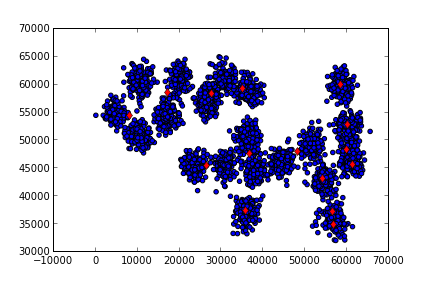
\includegraphics[height=4cm]{kmeans_2.png}

K-Means'i 20 kere işlettik. Eğer istenirse (hatta daha iyi olur) döngü bir
\verb!while! içine konur ve bitiş için "stabilite şartı"
aranır. Stabilite yeni küme merkezinin eskisinden "çok fazla değişik olup
olmadığı" şartıdır, değişim yoksa artık sonucu bulmuşuz demektir, daha
fazla döngüye gerek kalmayacaktır. Biz döngüyü 20 kere döngüyü işlettik,
bu problem için yeterli oldu.

K-Means işini bitirdikten sonra elde edilen sonuçları okuyabiliriz. Nihai
küme merkezleri \verb!/tmp/centers.csv! içinde. Bu merkezleri alıp,
ham veri üzerinde kırmızı nokta olarak gösteriyoruz.

veriyi 20-30 makinaya dağıtarak parça parça işleyip kümelemeniz
mümkündür. Endüstride son zamanlarda habire duyulan Büyük Veri (Big Data)
olayı işte bu.

\end{document}
